
\documentclass[12pt]{article}
\pagestyle{empty}
\setlength{\parskip}{0in}
\setlength{\textwidth}{6.8in}
\setlength{\topmargin}{-.5in}
\setlength{\textheight}{9.3in}
\setlength{\parindent}{0in}
\setlength{\oddsidemargin}{-.7cm}
\setlength{\evensidemargin}{-.7cm}

\usepackage{amsmath}
\usepackage{amsthm}
\usepackage{amstext}

\usepackage{graphicx}

\begin{document}


{\bf MAT 105 Quiz 1.1-1.4 (grey) Fall 2009} \hspace{.4in} {\large Name} \hrulefill

\hrulefill

 \emph{Relax.  You have done problems like these before.  Even if these problems look a bit different, just do what you can.  If you're not sure of something, please ask! You may use your calculator.  Please show all of your work and write down as many steps as you can.  Don't spend too much time on any one problem.  Please leave the following grading key blank for me to use.  Do well.  And remember, ask me if you're not sure about something.}

\begin{center}

\begin{tabular}
{|l|c|c|c|c|c|c|c|c|c|c|c|c|} \hline

 Problems & \hspace{5 pt} 1 \hspace{5 pt}  & \hspace{5 pt} 2 \hspace{5 pt} & \hspace{5 pt} 3 \hspace{5 pt} & \hspace{5 pt} 4 \hspace{5 pt} &  \hspace{5 pt} Total  \hspace{5 pt} & &  \hspace{5 pt} Grade \hspace{5 pt}  \\ \hline
&&&&& &&\\  
Points &&&&& &    \hspace{.8in}\% &  \\ 
&&&&& && \\  \hline
Out of & 16 & 16 & 6 & 12 &50 & & \\ \hline

\end {tabular}

\end{center}

\hrulefill

\begin{enumerate}

%%% Old 1.1-1.2, biology (baby), everyday
\item When my niece was born last year she weighed approximately 6 pounds.  After she was born, she gained 0.5 pounds per week.

\begin{enumerate}
\item Identify and name the variables in the story and state their units.
\vfill
\item Which variable is independent and which is dependent?
\vfill
\item Make a table showing my niece's weight after 2 weeks, 4 weeks, and 12 weeks.
\vfill
\vfill
\vfill
\item Is the function increasing or decreasing?
\vfill
\end{enumerate}

\newpage

%%% Old 1.2-1.3, home, everyday
\item The table shows the cost to hire a sod roller from the local home improvement center.  

\begin{center}
\begin{tabular} {|c|c|c|c|c|} \hline
$H$ & 1 & 5 & 12 & 24 \\ \hline
$C$ & 10 & 18 & 22 & 25 \\ \hline
\end{tabular}
\end{center}

In the table, $H$ = number of hours rented and $C$ = total cost of sod roller  (\$).

\begin{enumerate}
\item What is the cost for renting the roller for five hours?

\emph{Don't forget the units.}
\vfill
\item Approximately what is the cost for renting the sod roller for 20 hours?
\vfill
\item Draw a graph illustrating this information.  \emph{Be sure your axes are labeled and evenly scaled.  Plot the points given and sketch in a smooth line or curve connecting them.}

\vfill
\begin{center}
\scalebox {.8} {
\includegraphics [width = 6in] {graphPaper.pdf}}
\end{center}
\vfill

\item Does your answer to part b agree with your graph?  (Yes or no)  If no, what would a better answer be?
\vfill
\end{enumerate}

\newpage

%%% Old 1.3, pop culture, fun
\item The song ``Boom Boom Pow'' by Black Eyed Peas is off the hook!  The graph below shows its ranking on the ARC Weekly Top 40 Countdown.  The song entered the countdown on March 14, 2009.


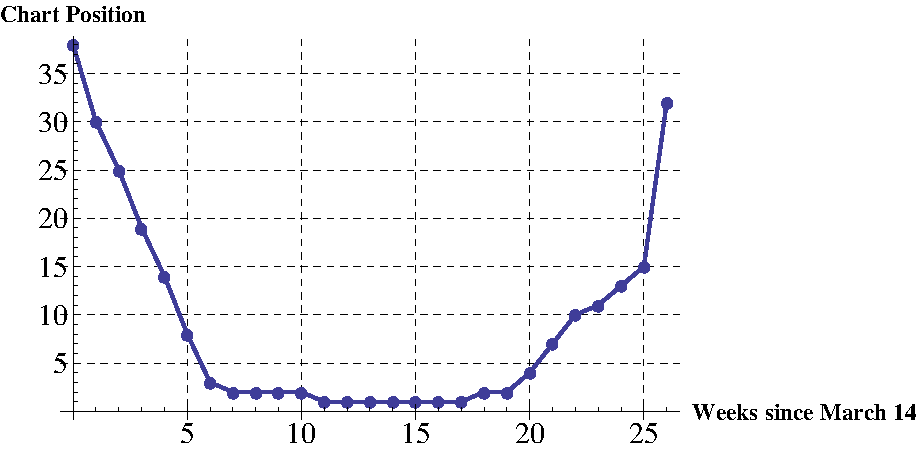
\includegraphics [width = 6in] {boomBoomPow}

\begin{enumerate}
\item After 22 weeks on the chart, what was the approximate ranking of the song?
\vfill
\item How many weeks did it take for the song to enter the top 10?
\vfill
\item Between the last two weeks on the chart, the song's position changed 17 positions.  What do you think caused such a rapid drop in the rankings?  Please write a sentence explaining your answer.
\vfill
\end{enumerate}

\newpage

%%% old 1.4, sports, fun
\item Shani Davis is a competitve skater from the U.S. who is one athlete to watch at the 2010 Vancouver Olympic Games.  He currently holds the world record in the 1500 meter race.  On March 6, 2009, he skated 1500 meters meters with a time of 1 minute and 41.80 seconds.

\begin{enumerate}
\item Convert his time into (decimal) minutes.
\vfill
\vfill
\item His speed was approximately 884 meters/minute, as you can check.  How fast did he skate in miles per hour?  \emph{Use 1 meter = 3.28 feet and 1 mile = 5,280 feet.}
\vfill
\vfill
\vfill
\end{enumerate}

\end{enumerate}

\end{document}
